\documentclass[border=12pt]{standalone}
\usepackage{tikz}
\usetikzlibrary{shapes.geometric, arrows.meta, positioning, calc, fit, backgrounds}
\usepackage{fontspec}
\setmainfont{DejaVu Sans}

\begin{document}
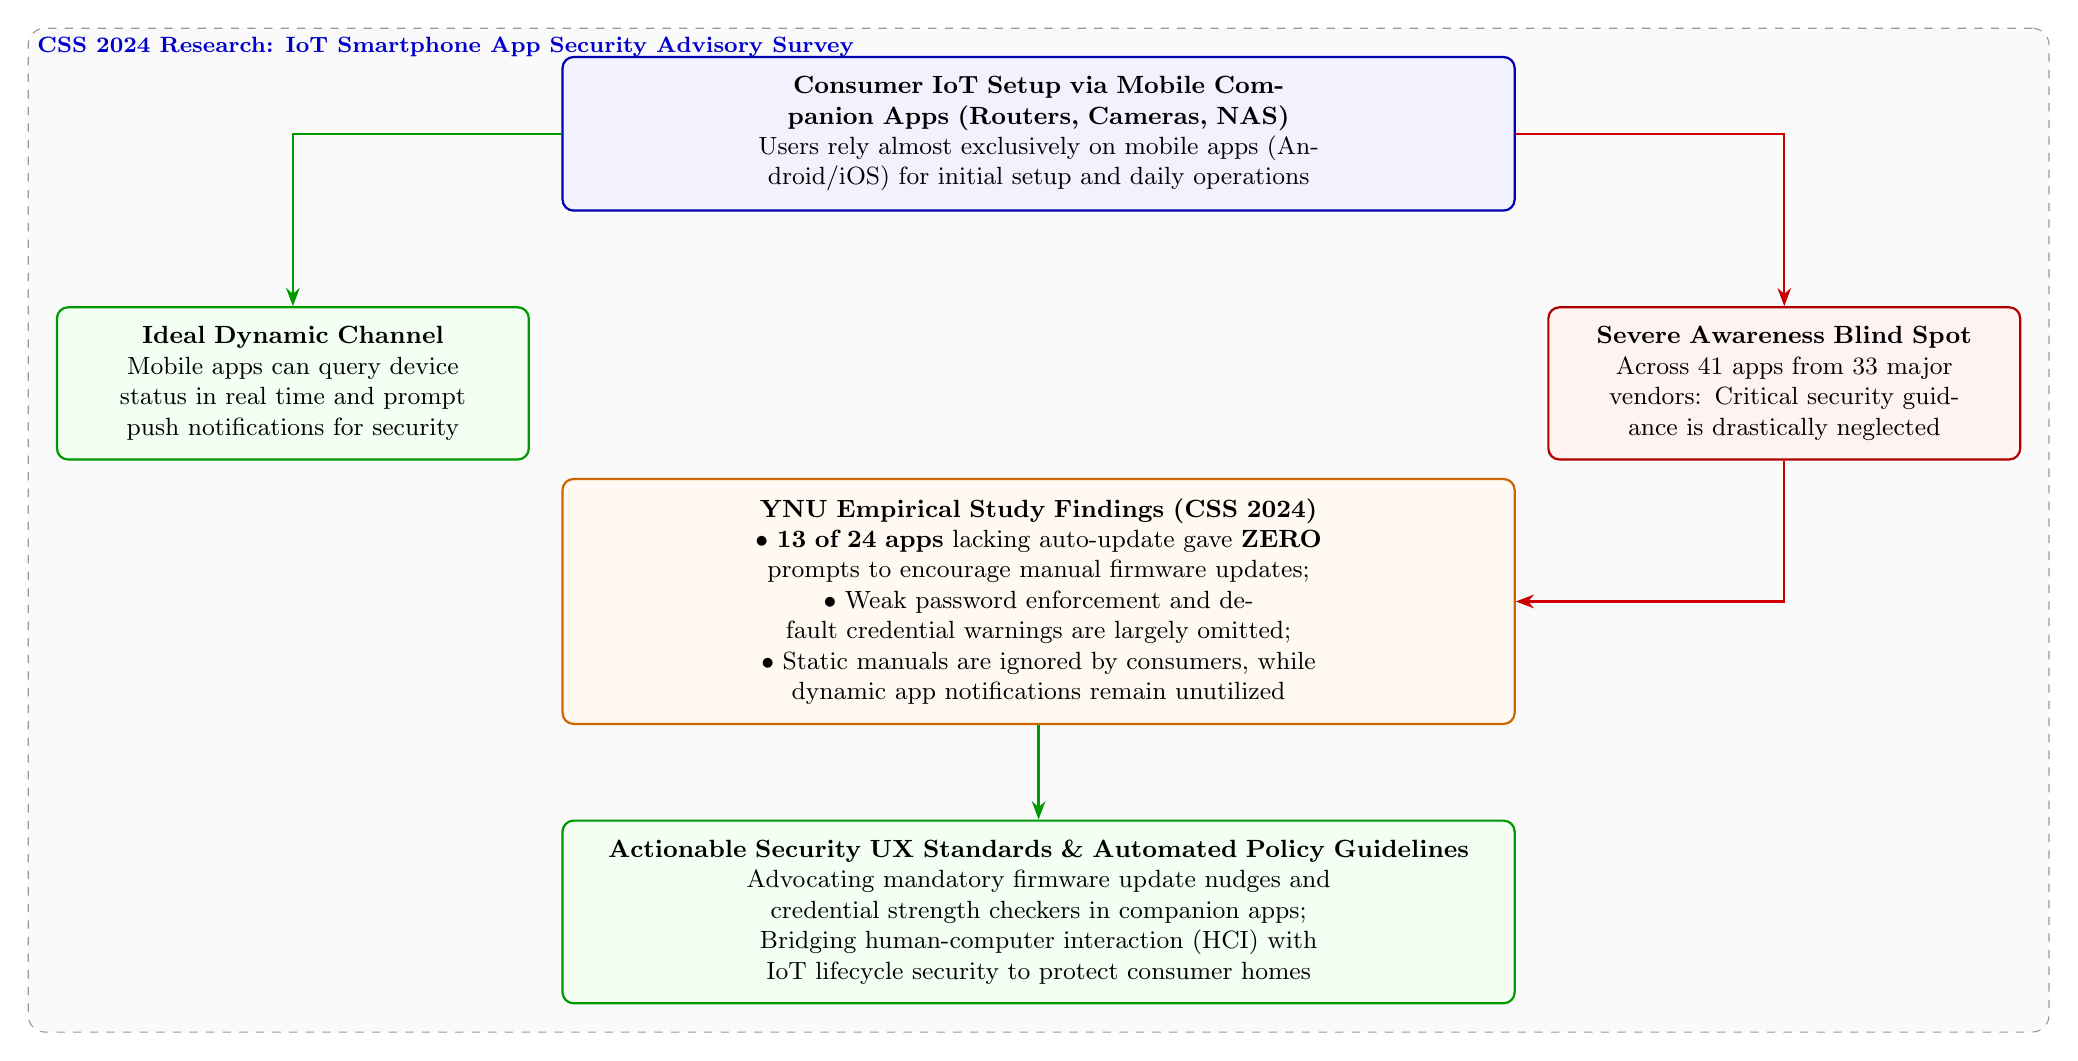
\begin{tikzpicture}[
    font=\small,
    >=Stealth,
    node distance=1.2cm,
    block/.style={rectangle, draw=blue!70!black, fill=blue!5, rounded corners=4pt, thick, align=center, inner sep=7pt},
    alertblock/.style={rectangle, draw=red!70!black, fill=red!5, rounded corners=4pt, thick, align=center, inner sep=7pt},
    greenblock/.style={rectangle, draw=green!60!black, fill=green!5, rounded corners=4pt, thick, align=center, inner sep=7pt},
    amberblock/.style={rectangle, draw=orange!80!black, fill=orange!5, rounded corners=4pt, thick, align=center, inner sep=7pt},
    groupbox/.style={draw=black!40, dashed, rounded corners=6pt, fill=black!2, inner sep=10pt}
]

    % Top: The Setup Dilemma in Consumer IoT
    \node[block, text width=11.6cm] (setup) {\textbf{Consumer IoT Setup via Mobile Companion Apps (Routers, Cameras, NAS)}\\Users rely almost exclusively on mobile apps (Android/iOS) for initial setup and daily operations};

    % Left: Theoretical Channel Advantage
    \node[greenblock, below left=1.2cm and 0.4cm of setup, text width=5.5cm] (potential) {\textbf{Ideal Dynamic Channel}\\Mobile apps can query device status in real time and prompt push notifications for security};

    % Right: Reality Check (YNU CSS 2024 Study)
    \node[alertblock, below right=1.2cm and 0.4cm of setup, text width=5.5cm] (reality) {\textbf{Severe Awareness Blind Spot}\\Across 41 apps from 33 major vendors: Critical security guidance is drastically neglected};

    \draw[->, thick, green!60!black] (setup) -| (potential);
    \draw[->, thick, red!80!black] (setup) -| (reality);

    % Middle: Empirical Findings via APK Reverse Engineering
    \node[amberblock, below=1.2cm of $(potential)!0.5!(reality)$, text width=11.6cm] (findings) {\textbf{YNU Empirical Study Findings (CSS 2024)}\\$\bullet$ \textbf{13 of 24 apps} lacking auto-update gave \textbf{ZERO} prompts to encourage manual firmware updates;\\$\bullet$ Weak password enforcement and default credential warnings are largely omitted;\\$\bullet$ Static manuals are ignored by consumers, while dynamic app notifications remain unutilized};

    \draw[->, thick, red!80!black] (reality) |- (findings);

    % Bottom: Recommendation for Secure App Ecosystems
    \node[greenblock, below=1.2cm of findings, text width=11.6cm] (policy) {\textbf{Actionable Security UX Standards \& Automated Policy Guidelines}\\Advocating mandatory firmware update nudges and credential strength checkers in companion apps;\\Bridging human-computer interaction (HCI) with IoT lifecycle security to protect consumer homes};

    \draw[->, thick, green!60!black] (findings) -- (policy);

    \begin{scope}[on background layer]
        \node[groupbox, fit=(setup) (potential) (reality) (findings) (policy), label={[anchor=north west, font=\footnotesize\bfseries, blue!80!black]north west:CSS 2024 Research: IoT Smartphone App Security Advisory Survey}] {};
    \end{scope}

\end{tikzpicture}
\end{document}
